\chapter{Лабораторная работа №4}

\textbf{Смирнов Пётр, ИУ7-65Б}

\section{Номер 1}

Чем принципиально отличаются функции cons, list, append?

cons создает списковую ячейку и расставляет указатели на голову и хвост, 
передается 2 S-выражения;

list создает столько списковых ячеек, сколько аргументов;

append выстраивает в одну цепочку элементы всех списков, 
поставляемых в качестве аргументов. append объединяет элементы 
списков, расположенные лишь на самом верхнем уровне. append 
создаёт копии все списков, кроме последнего.

Каковы результаты вычисления следующих выражений?

\begin{figure}[H]
    \begin{listingbox}{}
        \lstinputlisting[language=Lisp]{../1.lisp}
    \end{listingbox}
    \label{lst:1}
\end{figure}

\section{Номер 2}

Каковы результаты вычисления следующих выражений и почему?

LAST возвращает последние N ячеек списка. Если N не указано, 
возвращается последняя списковая ячейка.

REVERSE переставляет элементы в обратном порядке.

\clearpage

\begin{figure}[H]
    \begin{listingbox}{}
        \lstinputlisting[language=Lisp]{../2.lisp}
    \end{listingbox}
    \label{lst:2}
\end{figure}

\section{Номер 3}

Написать, по крайней мере, два варианта функции, которая 
возвращает последний элемент своего списка-аргумента.

\begin{figure}[H]
    \begin{listingbox}{}
        \lstinputlisting[language=Lisp]{../3.lisp}
    \end{listingbox}
    \label{lst:3}
\end{figure}

\section{Номер 4}

Написать, по крайней мере, два варианта функции, которая 
возвращает свой список-аргумент без последнего элемента.

\begin{figure}[H]
    \begin{listingbox}{}
        \lstinputlisting[language=Lisp]{../4.lisp}
    \end{listingbox}
    \label{lst:4}
\end{figure}

\section{Номер 5}

Напишите функцию swap-first-last, которая переставляет 
в списке-аргументе первый и последний элементы.

\begin{figure}[H]
    \begin{listingbox}{}
        \lstinputlisting[language=Lisp]{../5.lisp}
    \end{listingbox}
    \label{lst:5}
\end{figure}

\section{Номер 6}

Написать простой вариант игры в кости, в котором бросаются две
правильные кости. Если сумма выпавших очков равна 7 или 11 -- выигрыш,
если выпало (1, 1) или (6, 6) -- игрок имеет право снова бросить 
кости, во всех остальных случаях ход переходит ко второму игроку,
но запоминается сумма выпавших очков. Если второй игрок не 
выигрывает абсолютно, то выигрывает тот игрок, у которого больше очков.
Результат игры и значения выпавших костей выводить на экран с помощью
функции print.

\begin{figure}[H]
    \begin{imagebox}
        \centering
        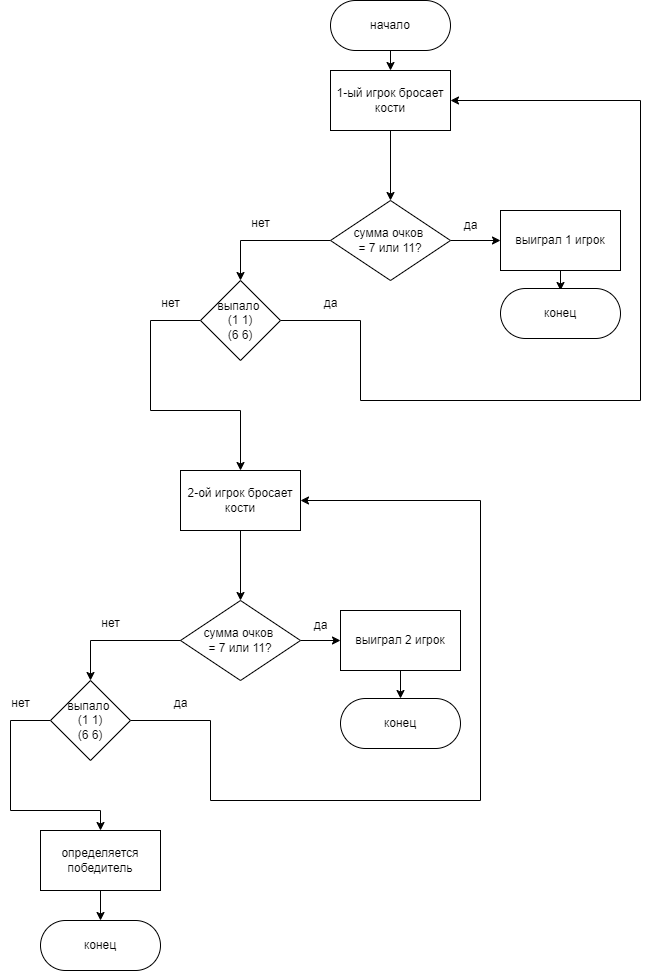
\includegraphics[width=0.8\textwidth]{../6.drawio.png}
    \end{imagebox}
    \caption{Схема алгоритма игры в кости.}
\end{figure}

\begin{figure}[H]
    \begin{listingbox}{}
        \lstinputlisting[language=Lisp]{../6.lisp}
    \end{listingbox}
    \label{lst:6}
\end{figure}

\section{Номер 7}

Написать функцию, которая по своему списку-аргументу lst 
определяет, является ли он палиндромом.

\begin{figure}[H]
    \begin{listingbox}{}
        \lstinputlisting[language=Lisp]{../7.lisp}
    \end{listingbox}
    \label{lst:7}
\end{figure}

\section{Номер 8}

Напишите свои необходимые функции, которые обрабатывают таблицу
из 4-х точечных пар: (страна.столица), и возвращают по стране --
столицу, а по столице -- страну.

\begin{figure}[H]
    \begin{listingbox}{}
        \lstinputlisting[language=Lisp]{../8.lisp}
    \end{listingbox}
    \label{lst:8}
\end{figure}

\section{Номер 9}

Напишите функцию, которая умножает на заданное число-аргумент
первый числовой элемент списка из заданного 3-х элементного 
списка-аргумента, когда а) все элементы списка -- числа,
б) элементы списка -- любые объекты.

\begin{figure}[H]
    \begin{listingbox}{}
        \lstinputlisting[language=Lisp]{../9.lisp}
    \end{listingbox}
    \label{lst:9}
\end{figure}